\chapter{Einleitung}

\section{Motivation}
Seit kurzem ist die E-Mobilität unter anderem ein neuer schulautonomer Schwerpunkt in der Abteilung Elektrotechnik, an der HTBLuVA-Salzburg. Passend zu diesem Schwerpunkt ergab sich die Idee ein Projekt zum Bereich E-Mobilität zu realisieren, um zukünftige Schüler daran zu interessieren.
Die E-Mobilität umfasst Elemente aus der Mechanik, Elektrotechnik, Kunststofftechnik und Informatik, das Projekt sollte so viele wie möglich  davon abdecken und darstellen können. Gleichzeitig soll das Projekt, eine Art von Prototyp für neu entwickelte Elektromotorräder sein und nicht nur als Abschlussprojekt dienen.

Das Umdenken der Gesellschaft von Verbrennungsmotoren auf Elektromotoren hat zur Folge, dass alltägliche Maschinen immer öfter mit Elektromotoren ausgestattet werden. Motorräder in dieser Größenordnung sind bis dato nicht vorhanden oder erhältlich. Es sind einige Firmen mit der Entwicklung dieser beschäftigt und es werden immer öfter neue Produkte präsentiert, doch diese Zeitalter ist erst am Anfang und benötigt noch Zeit.

Für die Herstellung eines zugelassenen Motorrades ist der Umfang einer Diplomarbeit, aus zeitlichen, sowie budgetären Gründen nicht realisierbar und aus diesem Grund Ist diese Projekt ein Prototyp eines vielleicht zukünftigen Elektro-Sport-Motorades, welches die Verwirklichung des Systems wiedergeben soll.

\section{Zielsetzung}
Ziel dieses Projektes war ein funktionierendes Motorrad, ohne Licht, Hupe oder sonstigen Zusatzfunktionen. Es sollte einfach das System funktionieren, welches die Fortbewegung ermöglichen soll. Das Betriebssystem soll Funktionsfähig und die Versorgung über die Akkus sichergestellt sein. 

Am Ende soll ein fahrtüchtiges Elektromotorrad mit den selben Fähigkeit, wie das Original das Ergebnis sein. Das Gewicht sollte wenn möglich reduziert, aber niemals erhöht werden. Die Zulassung wird in den darauffolgenden Jahren mit der Erweiterung von Licht, Hupe, und so weiter in der Studienzeit erlangt werden. Diese Projekt soll das Interesse des Projektteams an einer Entwicklung eines solchen Produkts bei Firmen zeigen, um aus diesen Prototypen einmal ein Produkt werden lassen zu können.

Die Allgemeinen Funktionen sind die allbekannten. Fahren mit Spitzen bis zu 130 km/h, Bremsen, ABS. Bei elektrischen Antrieben kann die Bremsleistung beim bergabfahren wieder in den Akku eingespeist werden. Diese Funktion nennt sich Rekuperation und wird bei Elektroautos schon verwendet und soll natürlich auch bei dem Elektromotorrad vorhanden sein.
\newpage

\section{Topologie des Gesamtsystems}

%\begin{figure} [H]
%	\begin{center}
%		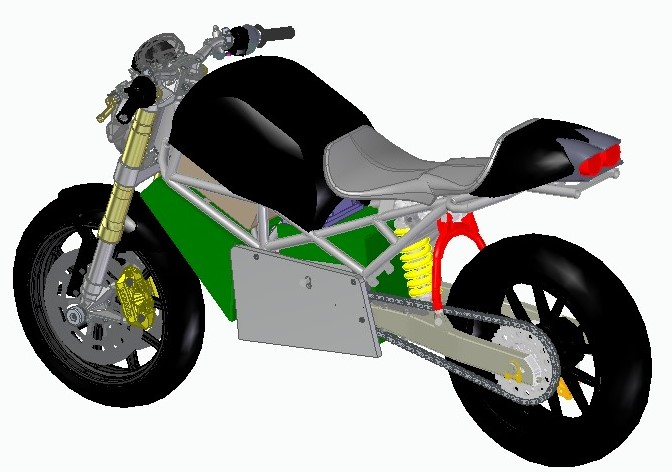
\includegraphics[scale=0.9] {figures/mechanik/Ducati1.jpg}
%		\caption{Topologiebild 1}
%		\label{fig:Topologiebild 1}
%	\end{center}
%\end{figure}
%
%
%\begin{figure} [H]
%	\begin{center}
%		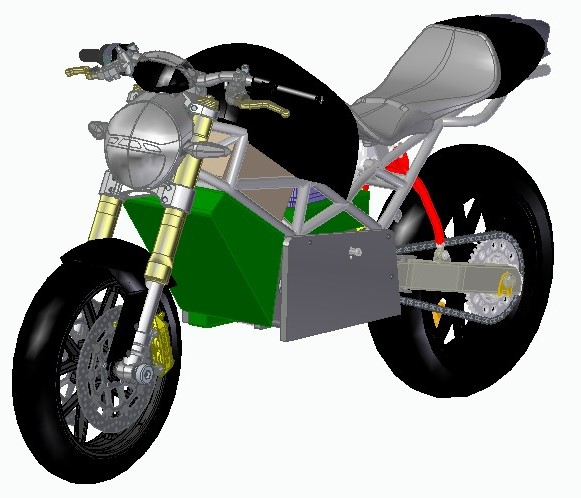
\includegraphics[scale=0.9] {figures/mechanik/Ducati2.jpg}
%		\caption{Topologiebild 2}
%		\label{fig:Topologiebild 2}
%	\end{center}
%\end{figure}

\newpage
\section{Leitfaden}

Die folgenden Kapitel dieses Dokuments beschreiben die verschiedenen Aspekte des Projekts im Detail. 

In Kapitel \ref{Stand der Technik} ist der Stand der Technik, der verwendeten Technologien, sowie kleinere Auszüge von Normen vorhanden. Dieses Kapitel soll einen Überblick über die Technologien gegeben. Auf dieses Kapitel folgen die Kapitel zur Beschreibung des "Emissionslosen Sportmotorrades". 

In Kapitel \ref{Mechanische Umsetzung} wird als erstes auf die mechanische Umsetzung von Gehäuse, Getriebe, Akkupacks, Akkukühlung und der Zusammenbau dieser Komponenten eingegangen. 

Kapitel \ref{Akku und Ladekonzept} handelt vom Akku- und Ladekozept, in dem eine Übersicht über die Aufgaben der Energieversorgung und des Batteriemanagement gegeben, sowie Die Energieversorgung dokumentiert ist. 

Anschließend beschreibt Kapitel \ref{Antriebsstrang} die Übersicht, den Hardwareaufbau,den Softwareaufbau und die Inbetriebnahme des Antriebsstranges und gibt Einblicke in die Entwicklung der Motorsteuerung. 

Als letztes wird in Kapitel \ref{Zentralsteuerung} Das Human-Computer-Interaction-System Beschrieben. Diese Kapitel beinhaltet die Beschreibung der Zentralsteuerung mit Fahrdatenspeicher, der Benutzeroberfläche am Display und Kommunikation mit der Motorsteuerung, die für den Betrieb entwickelt worden sind.

In nachfolgenden Teilbereichen gilt in den einzelnen Kapiteln eine interne Referenzierung auf einen Unterpunkt in selbigem Kapitel – heißt: „siehe Abschnitt 2.3“ bedeutet, dass besagter Punkt innerhalb des Kapitels nachzuschlagen ist.Wird allerdings auf Abschnitte oder Abbildungen verwiesen, die sich in einem anderen Kapitel befinden, so wird dies beispielsweise als „siehe Kapitel Stand der Technik Abschnitt 2.1.3“ angegeben. Die Namen der Kapitel sind dabei stets mit kursiver Schrift hervorgehoben, um eine bessere Lesbarkeit zu schaffen.